\documentclass[a4paper, 12pt]{article}
\usepackage[francais]{babel}
\usepackage{fontspec}
\usepackage{enumitem}
\usepackage{authblk}
\usepackage{minted}
\usepackage{amsmath}
\usepackage{hyperref}
\usepackage{tabularx}
\usepackage{multirow}
\usepackage{wrapfig}
\newcolumntype{C}[1]{>{\centering\arraybackslash}p{#1}}
\setlength{\parindent}{0pt}
\usepackage{hyperref}
\hypersetup{
    colorlinks,
    citecolor=black,
    filecolor=black,
    linkcolor=black,
    urlcolor=blue
}
\usepackage{etoolbox}
\patchcmd{\thebibliography}{\section*{\refname}}{}{}{}
\usepackage[left=2.5cm,top=2.5cm,right=2.5cm,bottom=2.5cm]{geometry}
\usepackage{glossaries}
	\let\oldnewacronym\newacronym
	\newcommand*{\provideacronym}[3]{%
	  \ifglsentryexists{#1}{%
	  }{%
	    \oldnewacronym{#1}{#2}{#3}%
	  }%
	}
\makeglossaries

\title{RustOS \protect\\ Système d’exploitation en Rust}
\author{Orphée Antoniadis}
\affil{\small Projet de Bachelor - Prof. Florent Glück}
\affil{\small Hepia ITI 3\up{ème} année}
\date{Semestre de Printemps 2017-2018}

\begin{document}
\maketitle

\begin{figure}[!b]
	\centering
	\begin{minipage}{.5\textwidth}
		\centering
		
\includegraphics[width=.6\linewidth]{images/hepia.jpg}
	\end{minipage}%
	\begin{minipage}{.5\textwidth}
		\centering
		
\includegraphics[width=.6\linewidth]{images/hesso.jpg}
	\end{minipage}
\end{figure}
\newpage

\section*{Résumé}
Le but de ce projet est d’étudier le langage Rust, en particulier son utilisation
pour l’implémentation d’un système d’exploitation de type \textit{bare metal}. Le
langage Rust se révèle particulièrement intéressant en tant que digne successeur de C :
beaucoup plus robuste que ce dernier et potentiellement tout aussi rapide. La première
partie du projet sera de comprendre les paradigmes de programmation utilisés par
Rust ainsi que ses caractéristiques principales. Dans un deuxième temps, il s’agira
d’implémenter un système d’exploitation très simple, similaire à celui réalisé au
cours logiciel « Programmation système avancée » mais écrit en Rust plutôt qu’en C.

\newpage
\setcounter{tocdepth}{3}
\tableofcontents
\newpage
\listoffigures
\newpage

\section*{Remerciements}
\newpage

\section*{Convention typographique}
Lors de la rédaction de ce document, les conventions typographique ci-dessous ont
été adoptées.
\begin{itemize}[label=\textbullet]
	\item Tous les mots empruntés à la langue anglaise ont été écrits en \textit{italique}
	\item Toute référence à un nom de fichier (ou dossier), un chemin d’accès, une 
    utilisation de paramètre, variable, ou commande utilisable par l’utilisateur, 
    est écrite avec la police d’écriture \mintinline{rust}{Courier New}.
	\item Tout extrait de fichier ou de code est écrit selon le format suivant:
    \begin{minted}[linenos,frame=single,tabsize=4]{rust}
    fn main() {
        println!("Hello, world!");
    }
    \end{minted}
\end{itemize}
\newpage

\newacronym{os}{OS}{\textit{Operating System}}
\newacronym{elf}{ELF}{\textit{Executable and Linkable Format}}
\newacronym{gcc}{GCC}{\textit{GNU Compiler Collection}}
\newacronym{iso}{ISO}{\textit{International Organization for Standardization}}
\newacronym{vram}{VRAM}{\textit{Video Random Access Memory}}
\newacronym{grub}{GRUB}{\textit{GRand Unified Bootloader}}
\newacronym{bios}{BIOS}{\textit{Basic Input Output System}}
\newacronym{pc}{PC}{\textit{Personal Computer}}
\newacronym{mbr}{MBR}{\textit{Master Boot Record}}
\newacronym{gdt}{GDT}{\textit{Global Descriptor Table}}
\newacronym{idt}{IDT}{\textit{Interrupt Descriptor Table}}
\newacronym{vga}{VGA}{\textit{Video Graphics Array}}
\newacronym{pio}{PIO}{\textit{Port Input/Output}}
\newacronym{cpu}{CPU}{\textit{Central Processing Unit}}
\newacronym{IA-32}{IA-32}{\textit{Intel Architecture, 32-bit}}
\newacronym{ram}{RAM}{\textit{Random Access Memory}}
\newacronym{mmu}{MMU}{\textit{Memory Management Unit}}
\newacronym{ldt}{LDT}{\textit{Local Descriptor Table}}
\printglossary[type=\acronymtype,title={Acronymes}]
\newpage

%%%%%%%%%%%%%%%%%%%%%%%%%%%%%%%%%%%%%%%%%%%%%%%%%%%%%%%%%%%%%%%%%%
%%%%%%%%%%%%%%%%%%%%%%%%%%%%%%%%%%%%%%%%%%%%%%%%%%%%%%%%%%%%%%%%%%

\section{Introduction}
\subsection{Contexte}
% Rust
% Cours programmation avancée des systèmes

%%%%%%%%%%%%%%%%%%%%%%%%%%%%%%%%%%%%%%%%%%%%%%%%%%%%%%%%%%%%%%%%%%

\subsection{Objectif}

\newpage
%%%%%%%%%%%%%%%%%%%%%%%%%%%%%%%%%%%%%%%%%%%%%%%%%%%%%%%%%%%%%%%%%%
%%%%%%%%%%%%%%%%%%%%%%%%%%%%%%%%%%%%%%%%%%%%%%%%%%%%%%%%%%%%%%%%%%

\section{Analyse}

\newpage
%%%%%%%%%%%%%%%%%%%%%%%%%%%%%%%%%%%%%%%%%%%%%%%%%%%%%%%%%%%%%%%%%%
%%%%%%%%%%%%%%%%%%%%%%%%%%%%%%%%%%%%%%%%%%%%%%%%%%%%%%%%%%%%%%%%%%

\section{Conception}
\subsection{Environnement de développement}
La machine utilisée pour le développement du projet est un MacBook Pro avec un
processeur Intel à 3 GHz. Il a quand même fallut utiliser une machine virtuelle
(VMware) utilisant Linux (Ubuntu 16.04.4 LTS) pour la compilation. Ce choix a été
fait car il existe beaucoup plus de documentation sur l'implémentation de systèmes
d'exploitation sur Linux que sur Mac. Bien que Mac \acrshort{os} soit un système UNIX, les
exécutables générés sur cet environnement n'ont pas le même format que ceux générés
sur Linux qui sont au format \acrshort{elf}. Ceci rend le développement d'\acrshort{os} légèrement
différent sur Mac \acrshort{os}.

%%%%%%%%%%%%%%%%%%%%%%%%%%%%%%%%%%%%%%%%%%%%%%%%%%%%%%%%%%%%%%%%%%

\subsection{Technologies}
\subsubsection{Nasm}
Bien que le système d'exploitation développé devait être sur Rust, certaines parties
ont du être faites en assembleur car étant trop bas niveau pour le Rust. Ces éléments
seront décrits plus loin dans ce document. Nasm a été  utilisé pour compiler le
code assembleur x86 en \acrshort{elf} 32-bits. Nasm produit des fichiers objets pouvant être
liés à d'autres fichiers objets afin de créer un exécutable. \\

\subsubsection{Rustup}
Rust sera décrit plus en détails dans un prochain chapitre. Ce qu'il faut savoir
est que Rust est distribué sous trois versions différentes. La version \textit{stable},
la version \textit{beta} et la version \textit{nightly}. La version \textit{nightly}
possède plus de fonctionnalités mais sa stabilité n'est pas garantie. Cette version
a été utilisée pendant le développement du projet et l'utilitaire Rustup a été utilisé
pour son installation. Cet utilitaire permet de simplifier l'installation de Rust
quand on souhaite une version différente de la dernière version stable de Rust. \\

\subsubsection{Cargo et Xargo}
Lors du développement d'un système d'exploitation type \textit{bare metal}, on souhaite
s'affranchir de toute dépendance à une librairie externe. Tout doit être refait depuis
le début. Le code est donc compilé sans la bibliothèque standard (std). Rust a tout
de même besoin d'une base pour être compilé. Cette base est fournie par la librairie
\mintinline{rust}{core}. Cette librairie est minimale et permet de ne définir que
les primitives de Rust. Pour gérer les dépendences d'un projet Rust, il est conseillé
d'utiliser le gestionnaire de paquets cargo. Le problème est que cargo ne permet
pas de lier la librairie \mintinline{rust}{core} à un projet. Heureusement, un 
autre utilitaire basé sur cargo existe et permet d'installer par défaut la librairie
\mintinline{rust}{core} pour des projets sans bibliothèque standard. Cet utilitaire
se nomme xargo et est utilisé pour compiler le code Rust en fichiers objets \\

\subsubsection{QEMU}
Le compilateur \acrshort{gcc} a été utilisé pour \textit{linker} les fichiers
objet générés par nasm et xargo. \acrshort{gcc} génère un fichier au format \acrshort{elf}.
Pour utiliser ce fichier comme un système d'exploitation \textit{bootable}, il faut
en faire une image \acrshort{iso} \textit{bootable}. Pour se faire, l'utilitaire
\mintinline{rust}{genisoimage} est utilisé, couplé au \textit{bootloader} \acrshort{grub}.
L'image \acrshort{iso} est finalement exécutée par la machine virtuelle QEMU.
QEMU est une machine virtuelle pouvant émuler une architecture. Pour ce projet,
l'architecture i386 a été choisie afin d'émuler un processeur Intel 32-bits.

%%%%%%%%%%%%%%%%%%%%%%%%%%%%%%%%%%%%%%%%%%%%%%%%%%%%%%%%%%%%%%%%%%

\subsection{Architecture}

\newpage
%%%%%%%%%%%%%%%%%%%%%%%%%%%%%%%%%%%%%%%%%%%%%%%%%%%%%%%%%%%%%%%%%%
%%%%%%%%%%%%%%%%%%%%%%%%%%%%%%%%%%%%%%%%%%%%%%%%%%%%%%%%%%%%%%%%%%

\section{Rust}

\newpage
%%%%%%%%%%%%%%%%%%%%%%%%%%%%%%%%%%%%%%%%%%%%%%%%%%%%%%%%%%%%%%%%%%
%%%%%%%%%%%%%%%%%%%%%%%%%%%%%%%%%%%%%%%%%%%%%%%%%%%%%%%%%%%%%%%%%%

\section{Exécution du \textit{kernel}}
\subsection{Compilation}
Quand on veut compiler un simple code C en utilisant \acrshort{gcc} par
exemple, le compilateur passe par plusieurs étapes. Le préprocesseur génère d'abord
un fichier C en fonction des directives de préprocesseur. Ce fichier C est ensuite
compilé en code assembleur qui est lui même compilé en code objet. Le \textit{linker}
permet ensuite de lier les différents fichiers objets et générer un exécutable.
Nous avons déjà eu un aperçu des différentes étapes de la compilation d'un \acrshort{os}
de type \textit{bare metal} dans la partie 3.2. A la différence de la compilation
d'un code C, nous avons d'un côté du code assembleur et de l'autre du code Rust.
Nasm et cargo permettent tous deux de générer des fichiers objets. Il n'y a donc
que la dernière étape à effectuer ce que \acrshort{gcc} permet de faire avec
la commande suivante.
\begin{minted}[tabsize=4]{shell}
gcc $(OBJS) -T $(LINKER) -static -m32 -ffreestanding -nostdlib -o $@ $(RUST)
\end{minted}
Ici, \mintinline{shell}{$(OBJS)} représente les fichiers objets générés par
\mintinline{rust}{nasm}, \mintinline{shell}{$(LINKER)} est un fichier permettant
de faire l'édition des liens et \mintinline{shell}{$(RUST)} représente les fichiers
objets générés par Rust.\cite{ref42}

%%%%%%%%%%%%%%%%%%%%%%%%%%%%%%%%%%%%%%%%%%%%%%%%%%%%%%%%%%%%%%%%%%

\subsection{\textit{Linking}}
Nous avons vu dans la partie précédente que \acrshort{gcc} a besoin d'un fichier
pour faire l'édition des liens. Si ce fichier n'est pas donné, il en utilise un par
défaut. Le \textit{linker} permet de structurer le code par sections. Prenons
pour exemple le \textit{script} utilisé pour ce projet.

\begin{minted}[fontsize=\footnotesize,linenos,frame=single,tabsize=4]{c}
ENTRY(entrypoint)
SECTIONS {
  . = 1M;
  .boot ALIGN(4):
  {
    *(.multiboot)
  }
  .stack ALIGN(4):
  {
    *(.stack)
  }
  .text ALIGN(4K) :
  {
    *(.text*)
  }
  .rodata ALIGN(4K) :
  {
    *(.rodata*)
  }
  .data ALIGN(4K) :
  {
    *(.data*)
  }
  .bss ALIGN(4K) :
  {
    *(COMMON)
    *(.bss*)
  }
}
\end{minted}

L'appel à \mintinline{c}{ENTRY} permet de spécifier l'entrée du \textit{kernel}.
Pour un simple programme en C l'entrée serait le \textit{main}. Ici, ce sera
l'entrée de notre \textit{kernel} donc la première fonction exécutée au \textit{boot}.
\mintinline{text}{SECTION} va dire au linker où placer les parties du code. Par exemple, 
la section \mintinline{text}{.text} contiendra le code et la section \mintinline{text}{.data}
contiendra les variables initialisées \cite{ref42,ref9,ref10,ref11}. Voici donc la structure
du fichier \acrshort{elf} qui serait généré à l'aide de ce \textit{script}.

\begin{figure}[!h]
  \centering
  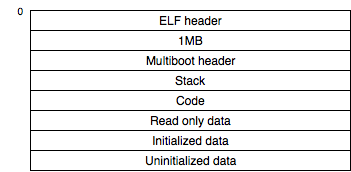
\includegraphics[scale=0.75]{images/elf_struct.png}
  \caption{Strucutre du fichier \acrshort{elf}}
\end{figure}

A noter que les sections commencent avec un \textit{offset} de 1MB. Nous avons eu
besoin de faire ça car les premiers 1MB dans un \acrshort{os} sont reservés \cite{ref42,ref13}.
La mémoire vidéo (\acrshort{vram}) se situe par exemple dans cette zone.

%%%%%%%%%%%%%%%%%%%%%%%%%%%%%%%%%%%%%%%%%%%%%%%%%%%%%%%%%%%%%%%%%%

\subsection{\textit{Boot}}
\subsubsection{Principe général}
Quand un ordinateur est allumé, un signal est envoyé à la carte mère qui démarre
l'alimentation. Le processeur démarre alors en mode 16-bits. Le signal "Power Ok"
est envoyé au \acrshort{bios} qui est le \textit{firmware} du \acrshort{pc}
(localisé en mémoire flash de la carte mère). Le \acrshort{bios} initialise alors
la séquence POST (\textit{Power On Self Test}) qui vérifie que chaque périphérique
est alimenté et que la mémoire est ok puis initialise chaque périphérique et enfin
redonne la main au \acrshort{bios} qui continue le \textit{boot}. Le \acrshort{bios}
charge ensuite les 512 premiers bytes (\acrshort{mbr}) du premier disque qui doit
charger le \textit{kernel} en mémoire et l'exécuter. Pour résumer, le \textit{boot}
d'une machine à base de \acrshort{bios} se déroule de la manière ci-dessous.\cite{ref42}

\begin{figure}[!h]
  \centering
  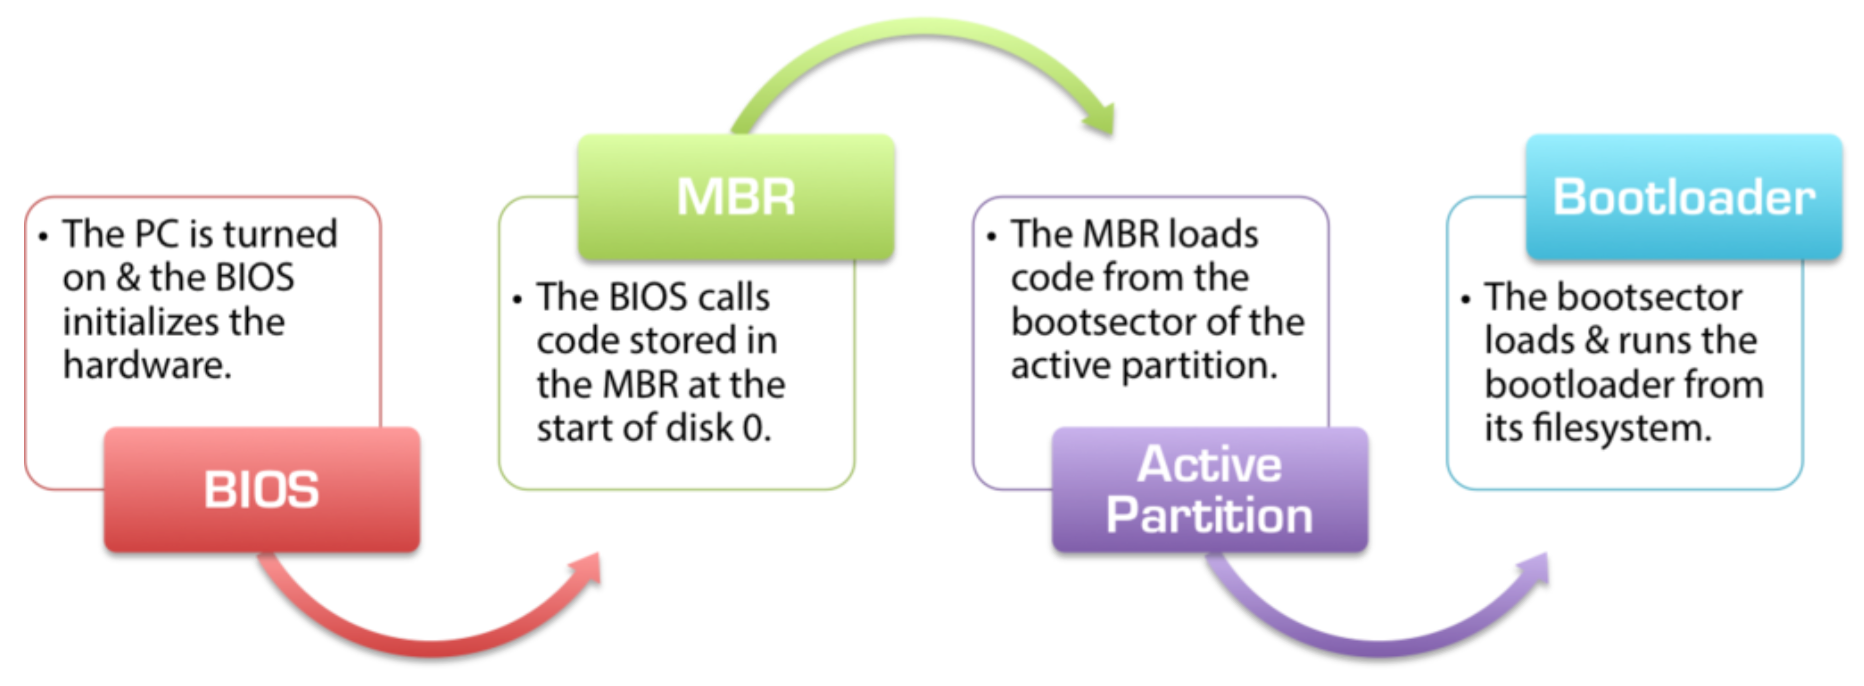
\includegraphics[scale=0.4]{images/bios_boot.png}
  \caption{\textit{Boot} d'une machine à base de \acrshort{bios}}
\end{figure}

\subsubsection{\acrshort{grub}}
Le \acrshort{mbr} contient ce qui est appelé le \textit{bootloader}. Le \textit{bootloader}
est le morceau de code qui va charger le \textit{kernel} en mémoire et l'exécuter.
C'est ici qu'entre en scène \acrshort{grub}. \acrshort{grub} est un \textit{bootloader}
puissant et versatile permettant de charger n’importe quel type de système d’exploitation.
Son initialisation se fait par étapes.
\begin{itemize}[label=\textbullet]
	\item \textit{Stage} 1: Chargé en mémoire par le \acrshort{bios} depuis le
    \acrshort{mbr}, il contient le code pour charger le \textit{Stage} 1.5
	\item \textit{Stage} 1.5: Chargé en mémoire par le \textit{Stage} 1, il contient
    les drivers nécessaires à l'accès au système de fichiers par le \textit{Stage} 2
	\item \textit{Stage} 2: Chargé en mémoire par le \textit{Stage} 1.5, il affiche
    le menu de \acrshort{grub}. Il permet de sélectionner et charger un \acrshort{os}
\end{itemize}

\acrshort{grub} permet de charger n'importe quel type de système d'exploitation
grace au standard \textit{Multiboot}. Ce standard permet à tout \textit{bootloader}
de charger tout \acrshort{os} compatible \cite{ref42,ref12}.

\subsubsection{Image \acrshort{iso}}
Nous avons déjà pu voir que le \textit{boot} du \textit{kernel} se faisait à partie
d'une image \acrshort{iso} dans la partie 3.2.4. Pour qu'une image \acrshort{iso}
soit \textit{bootable}, il est nécessaire que \acrshort{grub} soit installé dans
les huit premiers KB du disque. Prenons l'arborescence suivante :

\begin{minted}[tabsize=4]{shell}
isofiles
└── boot
    └── grub
\end{minted}

Les fichiers \mintinline{text}{kernel.elf} (kernel sur lequel nous voulons
\textit{booter}), \mintinline{text}{menu.lst} (fichier de configuration de \acrshort{grub})
et \mintinline{text}{stage2_eltorito} doivent être copiés de manière à obtenir
l'arborescence suivante :

\begin{minted}[tabsize=4]{text}
isofiles
└── boot
    ├── grub
    │   ├── menu.lst
    │   └── stage2_eltorito
    └── kernel.elf
\end{minted}

Pour finir, il faut exécuter la commande :
\begin{minted}[tabsize=4]{shell}
genisoimage -R -b boot/grub/stage2_eltorito -input-charset utf8 -no-emul-boot \
-boot-info-table -o os.iso isofiles
\end{minted}
Cette commande génerera une image \acrshort{iso} \textit{bootable} nommée \mintinline{text}{os.iso}\cite{ref42}.

\newpage
%%%%%%%%%%%%%%%%%%%%%%%%%%%%%%%%%%%%%%%%%%%%%%%%%%%%%%%%%%%%%%%%%%
%%%%%%%%%%%%%%%%%%%%%%%%%%%%%%%%%%%%%%%%%%%%%%%%%%%%%%%%%%%%%%%%%%

\section{Gestion mémoire}
\subsection{Introduction}
Le système d'exploitation développé est exécuté sur une architecture \acrshort{IA-32}
aussi appelée i386. Ceci qui veut dire que la mémoire est adressée sur 32 bits.
$2^{32}=4Go$, donc la mémoire physique (\acrshort{ram}) a une taille totale de
4Go dans notre système d'exploitation. Lorsqu'une tache est exécutée, elle est chargée
en mémoire et est définie par la paire base et limite. La base est son adresse physique
dans la \acrshort{ram} et la limite est sa taille. La figure \ref{ex_base_limit}
donne un exemple d'adressage de plusieurs processus.\cite{ref42}

\begin{figure}[!h]
  \centering
  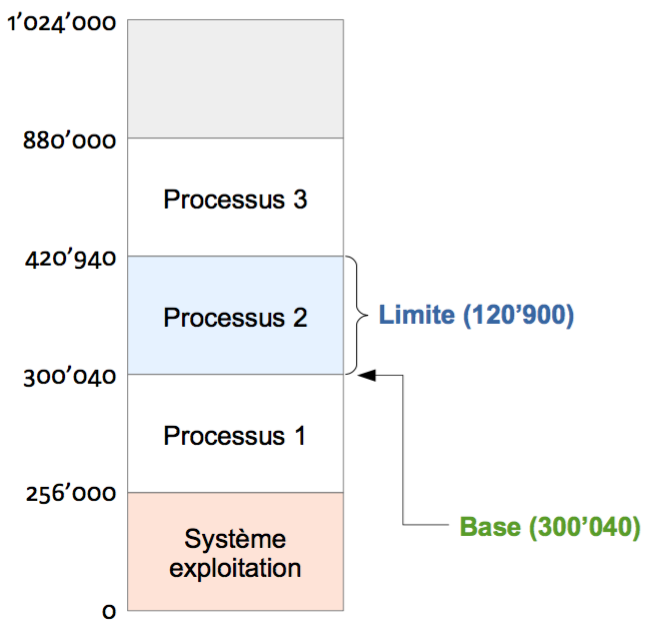
\includegraphics[scale=0.5]{images/ex_base_limit.png}
  \caption{Exemple d'adressage mémoire}
  \label{ex_base_limit}
\end{figure}

Une tache possède son propre espace d'adressage dit virtuel. Pour le processus 1
de la figure \ref{ex_base_limit}, l'adresse $0$ est en fait à l'adresse physique
$300040$. Il y a donc besoin de translater l'adresse virtuelle en adresse physique.
C'est là qu'entre en jeu le \acrshort{mmu} (Memory Mangement Unit). Le \acrshort{mmu}
est un dispositif matériel permettant de faire cette translation d'adresses. A chaque
référencement mémoire, il va convertir l'adresse virtuelle en adresse physique et
regarder si elle ne dépasse pas la limite du processus. Le \acrshort{mmu} permet donc
aussi de protéger la mémoire car il va empêcher toute référence à une zone extérieure
au processus (voir figure \ref{mmu}).\cite{ref42}

\begin{figure}[!h]
  \centering
  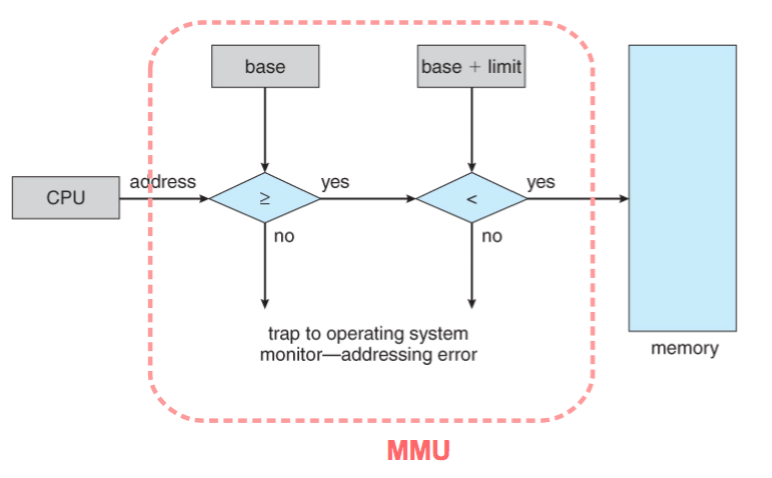
\includegraphics[scale=0.4]{images/mmu.png}
  \caption{Protection mémoire avec un \acrshort{mmu}}
  \label{mmu}
\end{figure}

%%%%%%%%%%%%%%%%%%%%%%%%%%%%%%%%%%%%%%%%%%%%%%%%%%%%%%%%%%%%%%%%%%

\subsection{\acrshort{gdt}}
Dans une architecture \acrshort{IA-32}, la translation d'adresses se fait à l'aide
de descripteurs définissant des segments de mémoire. Ces descripteurs sont contenus
dans une table de descripteurs. Cette table est la \acrshort{gdt} (Global Descriptor
Table) \cite{ref14}. Chaque descripteur est défini par sa base (son adresse physique),
sa limite (sa taille) et son niveau de privilèges (allant de 0 à 3, le niveau 0 
ayant le plus de privilèges et le niveau 3 le moins). Ci dessous, la figure \ref{gdt}
montre un exemple d'une \acrshort{gdt}.\cite{ref42}

\begin{figure}[!h]
  \centering
  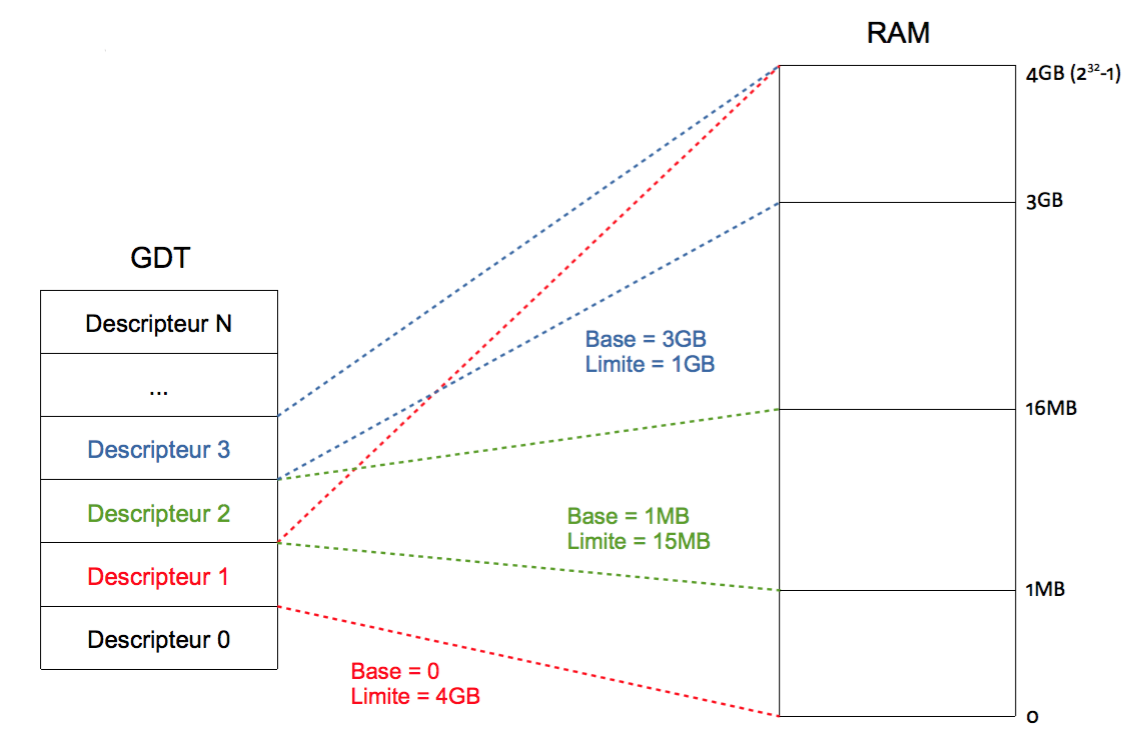
\includegraphics[scale=0.7]{images/gdt.png}
  \caption{Exemple d'une \acrshort{gdt}}
  \label{gdt}
\end{figure}

La \acrshort{gdt} est contenue en mémoire. Chaque entrée (ou descripteur) de
la table de descripteurs sont sur 64 bits et sont définis par la structure de
la figure \ref{gdt_entry}.\cite{ref14}

\begin{figure}[!h]
  \centering
  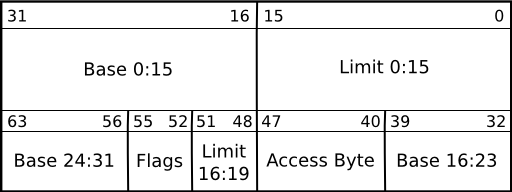
\includegraphics[scale=0.75]{images/gdt_entry.png}
  \caption{Structure d'une entrée dans la \acrshort{gdt}}
  \label{gdt_entry}
\end{figure}

\begin{itemize}[label=\textbullet]
	\item La base est sur 32 bits et est divisée en 3 parties dans une entrée.
    Les bits 16 à 31, 32 à 39 et 56 à 63 contiennent la base
	\item La limite est sur 20 bits et est divisée en 2 parties dans une entrée.
    Les bits 0 à 15 et 48 à 51 contiennt la limite
	\item L'\textit{Access byte} contient des bits de contrôle pour l'accès aux données
    du segment (privilèges, écriture ou lecture, etc...). Il est décrit plus en détails
    dans la figure \ref{gdt_bits}
    \item Les \textit{Flags} sont aussi des bits de contrôle et sont décrits plus
    en détails dans la la figure \ref{gdt_bits}\cite{ref14}
\end{itemize}

\begin{figure}[!h]
  \centering
  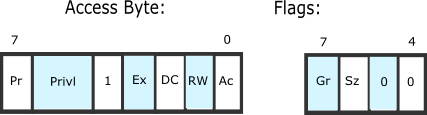
\includegraphics[scale=0.75]{images/gdt_bits.png}
  \caption{\textit{Access byte et Flags}}
  \label{gdt_bits}
\end{figure}

\begin{itemize}[label=\textbullet]
	\item Pr : \textit{Present} bit, doit être à 1 si le segment est valide
	\item Privl : Niveau de privilèges sur deux bits
	\item Ex : \textit{Executable bit}, est à 1 si le segment peut être exécuté
    (par exemple dans un segment de code, ce bit est à 1 alors que dans un segment
    de données, ce bit est à 0)
    \item DC : \textit{Direction bit}
    \item RW : Bit de lecture/ écriture
    \item Ac : \textit{Accessed bit}, ce bit est mis à 1 lorsque le \acrshort{cpu}
    accède à ce segment
    \item Gr : Bit de granularité, à 0 la limite est en octets, à 1 la limite est en blocs
    de 4Ko
    \item Sz : \textit{Size bit}, à 0 le segment est sur 16 bits, à 1 le segment
    est sur 32 bits
\end{itemize}

Par exemple, pour obtenir un segment sur toute la mémoire disponible, il faut mettre
le bit de granularité à 1 (pour avoir une limite en blocs de 4Ko) et mettre la
limite à 0xFFFFF. Une fois la \acrshort{gdt} construite, il faut utiliser l'instruction
\mintinline{text}{lgdt} pour la charger. L'adresse du descripteur de la \acrshort{gdt}
doit être donnée en argument à cette instruction. Le descripteur de \acrshort{gdt}
est défini par la structure 48-bits décrite dans la figure \ref{gdt_descriptor}.\cite{ref14}

\begin{figure}[!h]
  \centering
  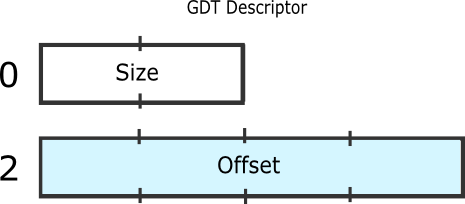
\includegraphics[scale=0.5]{images/gdt_descriptor.png}
  \caption{Descripteur de \acrshort{gdt}}
  \label{gdt_descriptor}
\end{figure}

\begin{itemize}[label=\textbullet]
	\item \textit{Size} est la limite sur 16 bits (c'est à dire la taille de la
    \acrshort{gdt} - 1)
	\item \textit{Offset} est l'adresse physique de la \acrshort{gdt} sur 32 bits
\end{itemize}

\newpage

%%%%%%%%%%%%%%%%%%%%%%%%%%%%%%%%%%%%%%%%%%%%%%%%%%%%%%%%%%%%%%%%%%

\subsection{Segmentation}
La segmentation est une technique permettant de découper la mémoire en segments
de mémoire logique. Une adresse logique est convertie par le \acrshort{mmu} en
adresse linéaire en utilisant une \acrshort{gdt} ou une \acrshort{ldt}.
Si la pagination (dont on parlera plus tard) est activée, l'adresse linéaire
est convertie en adresse physique. Toute cette mécanique est décrite dans la figure
\ref{addr_translation}. La segmentation permet de faire la convertion d'adresse
logique en adresse linéaire et est obligatoire en mode protégé (32-bits).\cite{ref17}

\begin{figure}[!h]
  \centering
  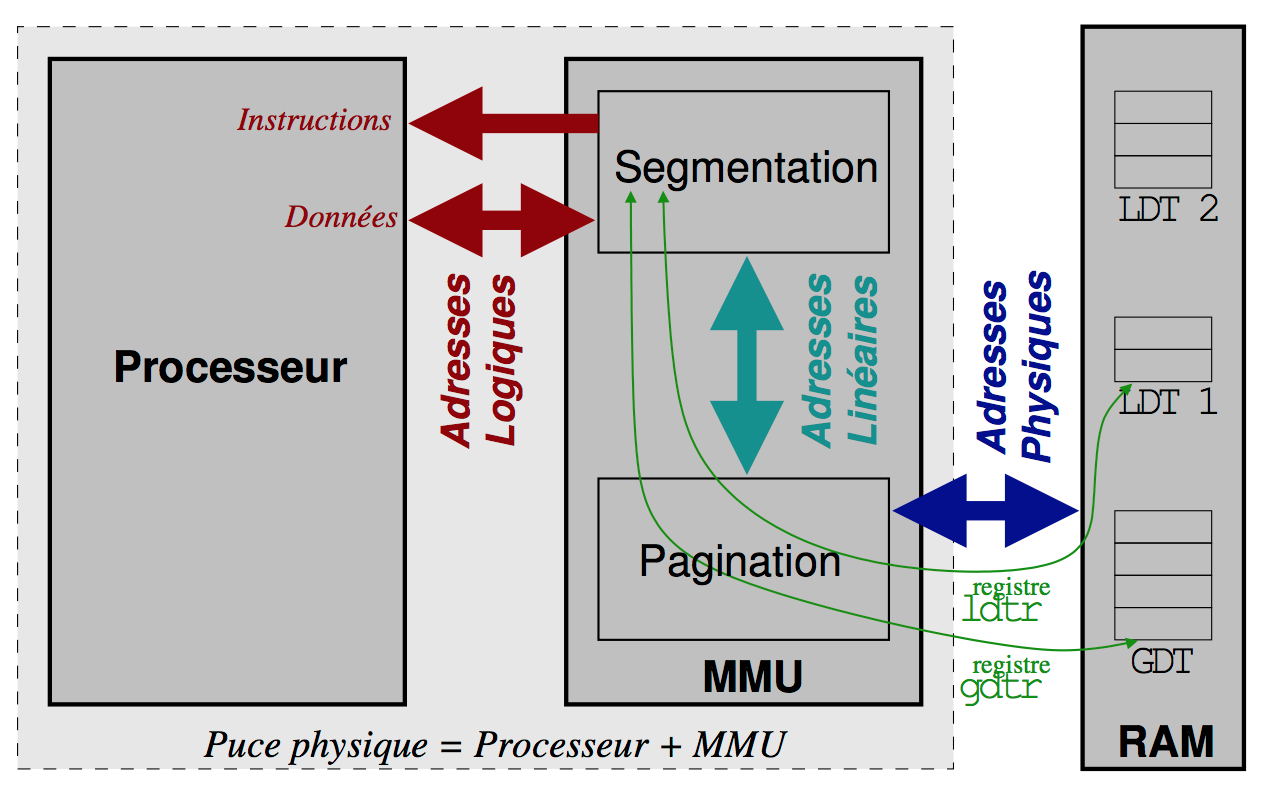
\includegraphics[scale=0.5]{images/addr_translation.png}
  \caption{Translation d'adresse}
  \label{addr_translation}
\end{figure}

La gestion de la segmentation par le \acrshort{cpu} se fait à l'aide de registres
spéciaux nommés registres de segment. Ces registres sont au nombre de 6 et ont
chacun une taille de 16 bits.\cite{ref42,ref18}

\begin{center}
	\scalebox{1}{
		\begin{tabular}{| C{5cm} | C{5cm} | }
			\hline
			Registre & Segment \\ \hline
			CS & \textit{Code Segment} \\ \hline
			DS & \textit{Data Segment} \\ \hline
			SS & \textit{Stack Segment} \\ \hline
			ES & \textit{Extra Segment} \\ \hline
			FS & \multirow{2}{*}{\textit{General Purpose Segments}} \\
            GS & \\ \hline
		\end{tabular}
	}
\end{center}

En mode protégé (32-bits), ces registres doivent pointer sur des descripteurs
de segment de la \acrshort{gdt}. Au minimum les trois premiers registres décrits
doivent être utilisé en mode protégé (CS, DS, et SS). Les opératons adressant le
code (décodage des instructons en mémoire, sauts, etc...) référencent le descripteur
de segment sur lequel pointe le registre CS. Les opératons adressant les données
(adressage de variables ou d'adresses mémoires) référencent le descripteur de segment
sur lequel pointe le registre DS. Les opératons adressant la pile (\mintinline{text}{push}
et \mintinline{text}{pop}) référencent le descripteur de segment sur lequel pointe
le registre SS. \\

Nous avons vu qu'un descripteur de segment fait 64 bits et un registre de segment
fait 16 bits. Ceci est possible car le registre de segment ne va pas contenir
l'integralité d'une entrée dans la \acrshort{gdt} mais un sélecteur de cette entrée.
Un sélecteur a une taille de 16 bits (comme les registres de segment) et contient
l'index du descripteur dans la \acrshort{gdt}, un bit indiquant si l'entrée est
dans la \acrshort{gdt} ou dans la \acrshort{ldt} ainsi que son niveau de privilège
(figure \ref{seg_sel}).\cite{ref42}

\begin{figure}[!h]
  \centering
  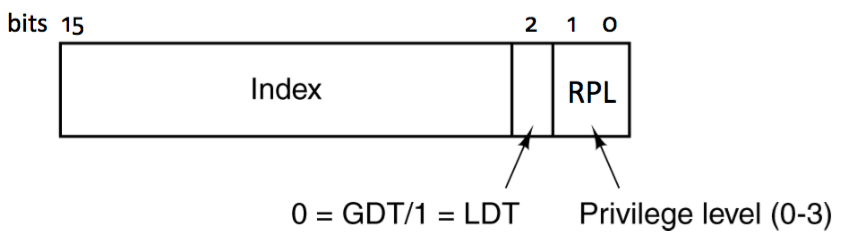
\includegraphics[scale=0.75]{images/seg_sel.png}
  \caption{Structure d'un sélecteur de segment}
  \label{seg_sel}
\end{figure}

Pour récupérer l'index dans la \acrshort{gdt} d'un segment à partir de son descripteur,
il faut donc faire un décallage de 3 bits. Prennons un segment si situant à l'index
2 de la \acrshort{gdt}. Si on veut initialiser le segment de code (registre CS)
avec ce segment, il faut mettre la valeur 16 dans le registre CS ($2 << 3 = 16$). \\

Dans un premier temps, l'\acrshort{os} développé a eu un adressage segmenté de type
\textit{FLAT}, c'est-à-dire que toute la mémoire était accédée de manière linéaire.
Ceci se fait en initialisant trois descripteurs dans la \acrshort{gdt}. Un descripteur
nul à l'index 0 (obligatoire dans touts les modèles de segmentation), un segment
de code couvrant toute la mémoire et un segment de données couvrant aussi toute la mémoire.
Les segments de code et de données adressent donc les mêmes zones de mémoire.
On verra par la suite que d'autres entrées ont été aujoutées à la \acrshort{gdt}
pour la gestion des tâches.

%%%%%%%%%%%%%%%%%%%%%%%%%%%%%%%%%%%%%%%%%%%%%%%%%%%%%%%%%%%%%%%%%%

\subsection{Pagination}
\subsubsection{Principe général}
La pagination est une autres techinque de gestion de mémoire qui diffère de la
segmentation. Alors que la segmentation permet d'allouer des morceaux de mémoire
de taille variable, la pagination divise la mémoire en blocs de taille fixe appelés
pages. De plus, la segmentation est obligatoire dans une architecture i386 alors que
la pagination ne l'est pas\cite{ref16}. Pour rappel, le mecanisme de segmentation
permet de convertir une adresse logique en adresse linéaire. Sur x86, lorsque la
pagination est activée, l'adresse linéaire est divisée en trois parties. 

\begin{itemize}[label=\textbullet]
	\item 10 bits pour le \textit{directory index}
	\item 10 bits pour le \textit{page index}
    \item 12 bits pour l'\textit{offset}
\end{itemize}

On dit que cette pagination est une pagination à trois niveaux. En général, une
pagination à trois niveaux est utilisée mais il peut exister des systèmes utilisant
plus de niveaux. Le système d'exploitation doit créer un répertoire (\textit{Page Directory})
et au moins une table de pages (\textit{Page Table}) pour chaque tâche. Quand une
adresse linéaire est lue, le \textit{directory index} permet de lire la bonne
entrée dans le \textit{Page Directory}. Cette entrée pointe sur la bonne page
dans la table des pages et c'est le \textit{page index} qui permet de récupérer
la bonne entrée dans cette page. Cette entrée pointe elle même sur la bonne page
dans les \textit{Page Frames} et l'\textit{offset} va être utilisé pour trouver
la donnée souhaitée. La figure \ref{paging3} résume bien ce mécanisme. A noter que le
\textit{Page Directory} est pointé par le registre CR3. A chaque fois qu'un changement
de tâche a lieu, le registre CR3 doit être mis à jour avec le \textit{Page Directory}
de la nouvelle tâche.\cite{ref15}

\begin{figure}[!h]
  \centering
  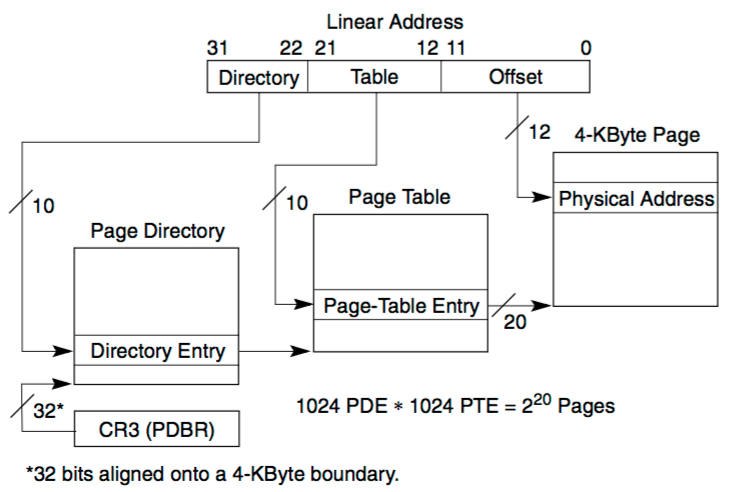
\includegraphics[scale=0.75]{images/paging3.png}
  \caption{Exemple de pagination à 3 niveaux}
  \label{paging3}
\end{figure}

\subsubsection{Activer la Pagination}
Pour initialiser la pagination sur architecture x86, il faut faire pointer le
registre CR3 vers un \textit{Page Directory} initial. Il faut donc commencer
par initialiser un \textit{Page Directory} "vierge" (qui ne pointe sur aucune 
table de pages). Chaque entrée de ce répertoire de pages doit être initialisé
à 0x2 (10 en binaire) car le bit 1 d'une entrée de page permet d'autoriser l'écriture
et la lecture. Il faut ensuite faire pointer la première entrée vers une table
de pages. La table de pages initiale se construit presque de la même manière
que le répertoire de pages sauf qu'il faut rajouter un bit d'attribut. Ce bit
est le bit 1 et indique que la page est utilisée. Toutes les pages dans la table
de pages doivent être utilisés donc toutes les entrées seront initialisées à 0x3
(11 en binaire).\cite{ref20} A noter qu'il faut mettre le bit 0 de la première entrée
du répertoire de pages à 1 aussi ce qui donne en rust :

\begin{minted}[fontsize=\footnotesize,tabsize=4]{rust}
    INITIAL_PAGE_DIRECTORY[0] = &INITIAL_PAGE_TABLE as *const _ as u32 | 0x3;
\end{minted}

Il n'est pas possible d'accéder au registre CR3 depuis le code rust, une fonction
assembleur qui a comme argument l'adresse vers le répertoire de pages initial doit
être appelée. Cette fonction effectue les instructions suivantes :

\begin{minted}[fontsize=\footnotesize,tabsize=4]{text}
    global enable_paging    ; Rend accessible la fonction depuis l'extérieur
    section .text:          ; Début de la section .text (code)
    enable_paging:
        mov eax,[esp+4]     ; Met l'adresse du répertoire de pages dans le registre eax
        mov cr3, eax        ; Fait pointer le registre cr3 sur le répertoire de pages
        
        mov ebx, cr0        ; Met le contenu du registre cr0 dans le registre ebx
        or  ebx, 1 << 31    ; Met le bit 31 du registre ebx à 1
        mov cr0, ebx        ; Met le contenu du registre ebx dans le registre cr0
        
        ret                 ; Retour de fonction
\end{minted}

\newpage
%%%%%%%%%%%%%%%%%%%%%%%%%%%%%%%%%%%%%%%%%%%%%%%%%%%%%%%%%%%%%%%%%%
%%%%%%%%%%%%%%%%%%%%%%%%%%%%%%%%%%%%%%%%%%%%%%%%%%%%%%%%%%%%%%%%%%

\section{Periphériques}
\subsection{Interruptions}
\subsubsection{Introduction}

\subsubsection{\acrshort{idt}}

%%%%%%%%%%%%%%%%%%%%%%%%%%%%%%%%%%%%%%%%%%%%%%%%%%%%%%%%%%%%%%%%%%

\subsection{Ports}
Les ports d'entrées/sorties sur architecture x86 se situent dans un espace d'adresses
séparé de la mémoire physique. Il n'est donc pas possible d'écrire dans un \acrshort{pio}
de la même manière que l'on écrirait dans la mémoire (avec une instruction 
\mintinline{text}{MOV}). Ainsi, le \acrshort{cpu} utilise des instructions speciales
pour accéder aux périphériques \acrshort{pio}. Ces instructions sont les instructions
\mintinline{text}{IN} et \mintinline{text}{OUT}. \mintinline{text}{IN} permet de lire
tandis que \mintinline{text}{OUT} permet d'écrire. A noter que l'adresse du port
doit toujours être spécifiée dans le registre \mintinline{text}{dx} et la lecture
et l'écriture se font toujours avec les registres \mintinline{text}{ax/al}.\cite{ref42}

%%%%%%%%%%%%%%%%%%%%%%%%%%%%%%%%%%%%%%%%%%%%%%%%%%%%%%%%%%%%%%%%%%

\subsection{\acrshort{vga}}
Dans l'\acrshort{os} développé, le mode texte \acrshort{vga} a été utilisé pour
l'affichage. Toute carte graphique offre ce mode texte de 80 colonnes par 25 lignes.
Les 16 couleurs disponibles sont les suivantes :\cite{ref19}
\begin{figure}[!h]
  \centering
  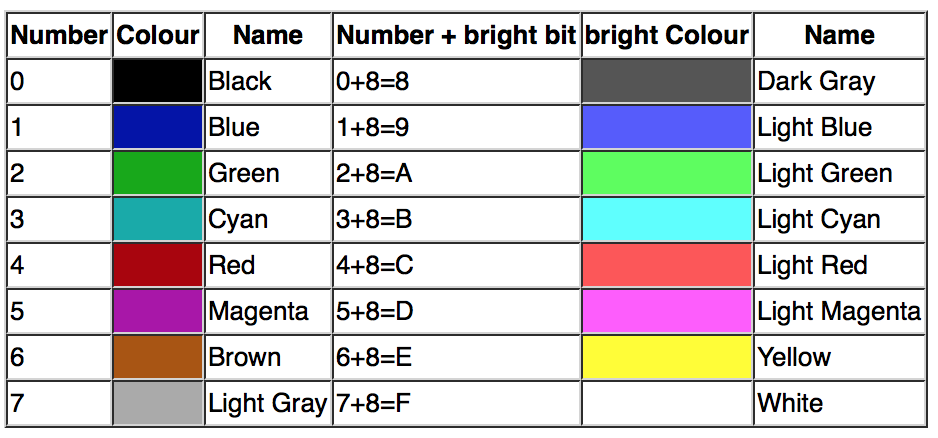
\includegraphics[scale=0.7]{images/colors.png}
  \caption{Couleurs du mode texte \acrshort{vga}}
\end{figure}

%%%%%%%%%%%%%%%%%%%%%%%%%%%%%%%%%%%%%%%%%%%%%%%%%%%%%%%%%%%%%%%%%%

\subsection{\textit{Timer}}

%%%%%%%%%%%%%%%%%%%%%%%%%%%%%%%%%%%%%%%%%%%%%%%%%%%%%%%%%%%%%%%%%%

\subsection{Clavier}

\newpage
%%%%%%%%%%%%%%%%%%%%%%%%%%%%%%%%%%%%%%%%%%%%%%%%%%%%%%%%%%%%%%%%%%
%%%%%%%%%%%%%%%%%%%%%%%%%%%%%%%%%%%%%%%%%%%%%%%%%%%%%%%%%%%%%%%%%%

\section{Système de fichiers}
\subsection{Introduction}

%%%%%%%%%%%%%%%%%%%%%%%%%%%%%%%%%%%%%%%%%%%%%%%%%%%%%%%%%%%%%%%%%%

\subsection{Structure}

\newpage
%%%%%%%%%%%%%%%%%%%%%%%%%%%%%%%%%%%%%%%%%%%%%%%%%%%%%%%%%%%%%%%%%%
%%%%%%%%%%%%%%%%%%%%%%%%%%%%%%%%%%%%%%%%%%%%%%%%%%%%%%%%%%%%%%%%%%

\section{Résultats}

\newpage
%%%%%%%%%%%%%%%%%%%%%%%%%%%%%%%%%%%%%%%%%%%%%%%%%%%%%%%%%%%%%%%%%%
%%%%%%%%%%%%%%%%%%%%%%%%%%%%%%%%%%%%%%%%%%%%%%%%%%%%%%%%%%%%%%%%%%

\section{Discussions}
\subsection{Problèmes rencontrés}

%%%%%%%%%%%%%%%%%%%%%%%%%%%%%%%%%%%%%%%%%%%%%%%%%%%%%%%%%%%%%%%%%%

\subsection{Améliorations possibles}

\newpage
%%%%%%%%%%%%%%%%%%%%%%%%%%%%%%%%%%%%%%%%%%%%%%%%%%%%%%%%%%%%%%%%%%
%%%%%%%%%%%%%%%%%%%%%%%%%%%%%%%%%%%%%%%%%%%%%%%%%%%%%%%%%%%%%%%%%%

\section{Conclusion}

\newpage
%%%%%%%%%%%%%%%%%%%%%%%%%%%%%%%%%%%%%%%%%%%%%%%%%%%%%%%%%%%%%%%%%%
%%%%%%%%%%%%%%%%%%%%%%%%%%%%%%%%%%%%%%%%%%%%%%%%%%%%%%%%%%%%%%%%%%

\section{Références}
\nocite{*}
\bibliographystyle{unsrt}
\bibliography{biblio}

\end{document}
